\documentclass[11pt,a4paper]{article}
\usepackage{acl2015}
\usepackage{url}
\usepackage{latexsym}
\usepackage{graphicx}

\title{Asignatura Text Mining II\\
M\'aster/Diploma Big Data Analytics}

\author{Pedro Henrique Mano Figueiredo Fernandes \\
  {\tt pedromorfeu@gmail.com} \\}

\date{\today}

\begin{document}
\maketitle
\begin{abstract}
  
  La aproximaci\'on al problema de {\em Text Mining} para {\em Author Profiling} ha tenido como base la t\'ecnica conocida por {\em bag of words}. Esta t\'ecnica emplea modelos para aprender el vocabul\'ario de un conjunto de documentos, a trav\'es del que se construye una representaci\'on de los datos en forma de matriz, adecuada para aplicar {\em machine learning}. A la matriz de vocabulario se han a\~nadido otras caracter\'isticas, como contadores de polaridad de sentimientos y determinadas estad\'isticas del texto de los documentos. El metadata de los tweets se ha usado también para reforzar las caracter\'isticas de la matriz.
  
  El modelo usado para el aprendizaje del vocabul\'ario se basa en contadores de palabras, calculando un coheficiente de tipo TF-IDF. Se ha configurado el modelo con un máximo de 2000 caracter\'isticas, que se traduce en el c\'alculo de las 2000 palabras más significativas en el corpus de entrenamiento. Para la divisi\'on de los documentos en trozos ({\em tokens}) se han aplicado {\em tokenizers} especializados en texto de Twitter.
  
  Una vez constru\'ida la matriz con todas las caracter\'isticas, se ha elegido un clasificador de tipo RandomForest para entrenar un modelo matem\'atico. Este clasificador es de tipo {\em ensemble}, aplicando varias iteraciones de predicci\'on sobre conjuntos aleat\'orios de los datos, lo que garantiza una mejor generalizaci\'on del modelo.

\end{abstract}


\section{Introducci\'on}

  La exploraci\'on de datos de lenguage natural permite descubrir caracter\'sticas de los autores basadas en sus patrones de escrita. El objectivo de este ejerc\'icio es explorar la informaci\'on de un dataset constitu\'ido por tweets de varios usuarios de distintos pa\'ises de habla hisp\'anica, con el intuito de crear un modelo clasificador de perfiles de sexo y pa\'is.
  
  Determinados patrones de escrita pueden mostrar ind\'icios de perfiles. Por ejemplo, los hombres tienen tendencia a usar m\'as determinantes y adjectivos que las mujeres; y las mujeres suelen usar m\'as pronombres y la negaci'on. En general, las mujeres tienen tendencia a demostrar m\'as carga emocional en sus frases que los hombres. M\'etricas como el tamaño de las frases pueden eventualmente ser significativas tambi\'en. Adem\'as, hay que tener en cuenta los usuarios corporativos, cuya escrita ser\'a diferente de la de otros perfiles, probablemente m\'as formal.
  
  De la misma forma, los perfiles de pa\'ises obedecen a patrones de escrita, con elementos significativos como el uso de modismos y otras variaciones lengu\'isticas. 
  
  El corpus de texto se usa para aprender el vocabul\'ario significativo y luego aplicar t\'ecnicas de {\em machine learning}, que se encargar\'an de encontrar patrones y correlaciones para generar un modelo matem\'tico. Los datos sirven como mat\'eria prima, a la que se aplican herramientas para crear nuevo conocimiento.


\section{Dataset}

  El dataset de este ejerc\'icio est\'a constitu\'ido por cientos de tweets de usuarios de 7 pa\'ises de habla hisp\'anica. Cada pa\'is tiene tweets de 650 usuarios y cada usuario tiene entre 600 y 1000 tweets. 
  
  El conjunto de entrenamiento cuenta con datos de 2730 usuarios previamente clasificados en sexo y pa\'is. En total hay 2.616.338 tweets, que constituye el corpus para calcular el vocabulario. El conjunto de test tiene 1820 usuarios y respectiva clasificaci\'on, con un total de tweets de 1.741.060. El volumen de datos es bastante grande y de c\'omputo exigente: en una m\'aquina con 4GB de RAM y un procesador i3, el c\'alculo del vocabulario para solamente 2000 palabras tarda m\'as de 10 minutos.
  
  Se ha realizado un breve an\'alisis estad\'istico sobre la matriz de {\em bag of words} con R, cuyos resultados se presentan a continuaci\'on. El gr\'afico siguiente representa las palabras y s\'imbolos con mayor coeficiente TF-IDF:
  
  \begin{figure}[ht!]
    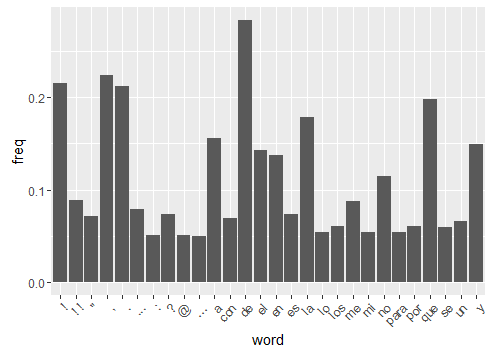
\includegraphics[width=\linewidth]{most_used_words.png}
    \caption{Palabras con mayor coeficiente TD-IDF.}
    \label{fig:most_used_words}
  \end{figure}
  
  Se verifica que las palabras m\'as significativas son tambi\'en las m\'as usuales.
  
  En un breve an\'alisis de sentimientos (positivo y negativo), se puede ver que la media es ligeramente superior en las mujeres.
  
  \begin{figure}[ht!]
    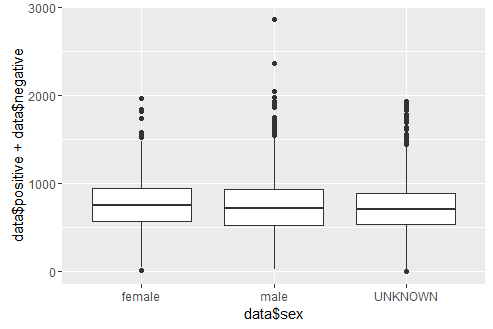
\includegraphics[width=\linewidth]{sentiment.png}
    \caption{Sentimiento.}
    \label{fig:sentiment}
  \end{figure}
  
  El tama\~no medio de frases muestra que los hombres escriben frases m\'as largas:

  \begin{figure}[ht!]
    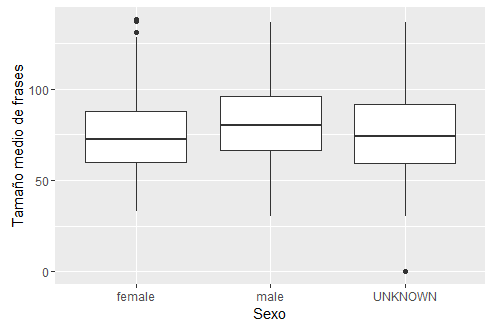
\includegraphics[width=\linewidth]{sentence_mean.png}
    \caption{Tama\~no medio de frases.}
    \label{fig:sentence_mean}
  \end{figure}
  
  
  Estad\'isticas del dataset que el alumno considere importantes. En clase se han visto las estad\'isticas b\'asicas del dataset y se ha explorado para obtener caracter\'isticas m\'as avanzadas. En este apartado el alumno tiene total libertad para exponer las tablas o gr\'aficas que considere apropiadas para describir el dataset, tanto desde un punto de vista ling¨u\'istico como de big data. 


\section{Propuesta del alumno}

Descripci\'on de la propuesta. Qu\'e caracter\'isticas se han utilizado y cu\'al ha sido la hip\'otesis para elegirlas. En clase se ha visto la construcci\'on de una baseline basada en bolsa de palabras. En este apartado el alumno expondr\'a las mejoras propuestas.

\section{Resultados experimentales}

Presentaci\'on de los resultados y an\'alisis de los mismos. La presentaci\'on de resultados y su an\'alisis implica mostrar en qu\'e contribuye la propuesta realizada, es decir, ¿son mejores los resultados?, ¿se procesan m\'as r\'apidos los datos?, ¿se aportan nuevas explicaciones conceptuales al problema?

\section{Conclusiones y trabajo futuro}

Breve presentaci\'on de las conclusiones sobre  el trabajo realizado e ideas de futuro para mejorar los resultados.


\begin{thebibliography}{}

\bibitem[\protect\citename{Aho and Ullman}1972]{Aho:72}
Alfred~V. Aho and Jeffrey~D. Ullman.
\newblock 1972.
\newblock {\em The Theory of Parsing, Translation and Compiling}, volume~1.
\newblock Prentice-{Hall}, Englewood Cliffs, NJ.

\end{thebibliography}

\end{document}
